%
% This work is licensed under a Creative Commons Attribution-ShareAlike 4.0 International License.
%

\documentclass[10pt, a5paper, twoside, openany]{memoir}

\setsecnumdepth{subsection}

\title{Introduction to Quantum Mechanics}
\author{Joseph D. MacMillan}
\date{}


\usepackage{graphicx}
\usepackage{color} 
\usepackage{amsmath, amssymb}
\usepackage{libertinus}
\usepackage{microtype}
\usepackage{layout}
\usepackage[most]{tcolorbox}
\tcbuselibrary{skins,breakable}
\usepackage[hang, small, bf]{caption}
\captionsetup[table]{position=top}
\captionsetup[figure]{position=bottom}
\usepackage[hyphens]{url}
\usepackage[hidelinks]{hyperref}
\hypersetup{pdftitle={Introduction to Quantum Mechanics}}
\hypersetup{pdfauthor={Joseph D. MacMillan}}
\urlstyle{rm}
\usepackage[shortlabels]{enumitem}


% Set page margins, etc
\setstocksize{9in}{6in}
\settrimmedsize{\stockheight}{\stockwidth}{*}
\settrims{0pt}{0pt}

\setlxvchars %define lenght 65 char of the used font
\settypeblocksize{*}{1.05\lxvchars}{1.7}
\setbinding{20pt} 
\setlength{\headheight}{30pt}
\setlength{\footskip}{20pt}

\setulmargins{90pt}{*}{*}
\setlrmargins{*}{*}{*}
\setheaderspaces{*}{30pt}{*}

\setmarginnotes{0.01pt}{20pt}{\onelineskip}
\checkandfixthelayout

\setcounter{tocdepth}{3}



\newcommand{\uu}{\symbfup{u}}
\newcommand{\grad}{\symbfup{\nabla}}
\newcommand{\curl}{\symbfup{\nabla} \times}
\newcommand{\dfdx}[2]{\frac{\partial {#1}}{\partial {#2}}}
\newcommand{\ddfdx}[2]{\frac{\partial^2 {#1}}{\partial {#2}^2}}
\newcommand{\vort}{\symbfup{\omega}}
\renewcommand\vec{\symbfup}
\newcommand{\unit}[1]{\hat{\vec{#1}}}
\newcommand{\U}{\mathbb{U}}
\newcommand{\V}{\mathbb{V}}
\newcommand{\LL}{\mathbb{L}^2}
\newcommand{\LLLL}{\mathbb{L}^4}

\newcommand{\ket}[1]{| #1 \rangle}
\newcommand{\bra}[1]{\langle #1 |}
\newcommand{\braket}[2]{\langle #1 | #2 \rangle}


%\DeclareMathAlphabet{\mathbfsf}{\encodingdefault}{\sfdefault}{bx}{sl}
\newcommand{\tens}[1]{\mathbfsfit{#1}}


\newcounter{example}[chapter]
\def\theexample{\thechapter.\arabic{example}}
\newenvironment{example}[1][ ]{\refstepcounter{example}
\begin{tcolorbox}[breakable, sharp corners, boxrule = 0pt, frame empty, opacityframe=0, parbox=false]
\textbf{Example \theexample \ -- #1.}
}
{ 
\end{tcolorbox}
}

\newenvironment{theorem}[1][ ]{
\begin{tcolorbox}[breakable, sharp corners, boxrule = 0pt, frame empty, opacityframe=0, parbox=false]
\textbf{#1.}
}
{ 
\end{tcolorbox}
}

\newcounter{problem}[chapter]
\def\theproblem{\thechapter.\arabic{problem}}
\newenvironment{problem}[1][ ]{\refstepcounter{problem} \noindent \textbf{Problem \theproblem \ -- #1.}}{\vspace{0.1in}}


\begin{document}

\frontmatter

\maketitle

\begin{center}


\includegraphics[width=\linewidth]{Figures/fig_cover_wave}

\vspace{1in}

{\small

This version was compiled on \today.  For the most up-to-date version and supplementary material, see \href{https://josephmacmillan.github.io/IntroductionToQuantumMechanics/index.html}{josephmacmillan.github.io/IntroductionToQuantumMechanics}.

\vspace{2in}

This work is licensed under a \href{https://creativecommons.org/licenses/by-sa/4.0/}{Creative Commons Attribution-ShareAlike 4.0 International License}.
}
\end{center}


\newpage

\tableofcontents

\chapter{Preface}

To come. 

\section{Why Open Education?}

This book and the supplementary material are released under a Creative Commons Attribution-ShareAlike 4.0 International License, which means you can do anything you want with this book:  cut out stuff you don't need, use it to build an even better book, download it for free off the web, print it out yourself, give it to your friends (they want a copy, trust me), and anything else you can think of.  The only stipulation is that you give credit where it's due, and release the derivative work under the same license.

Why did I choose this?  Because I've taught university courses and have seen the issues with expensive textbooks: students not being able to afford them, students finding illegal PDF copies online and sharing them, the publishing companies fighting back with various schemes like renting digital copes, and so on.  Especially in advanced physics, little textbooks can be so expensive, and yet I think textbooks are an important and necessary resource, and I want my students to all have a copy.

\section{Thanks}

To come.

\vspace{1in}

Find a typo, mistake, or horrible misconception in this book?  Let me know by creating a new issue at the GitHub page:  

\href{https://github.com/josephmacmillan/IntroductionToQuatumMechanics/issues}{github.com/josephmacmillan/IntroductionToQuantumMechanics/issues}.



\mainmatter

\chapter{The Stern-Gerlach Experiment}

\section{Spin Angular Momentum}

Let's start with a system that is pretty much as far away from the quantum world as possible -- the Earth and Sun, as shown in Figure \ref{fig_sun_earth}.  With its total motion, the Earth has two kinds of angular momentum:  \emph{orbital} angular momentum $\vec{L}$ from its orbit around the sun, and \emph{spin} angular momentum $\vec{S}$, resulting from its 24 hour rotation.  Of course, the spin angular momentum in this case is due to adding up the orbital angular momentum $\vec{L}_i = \vec{r}_i \times \vec{p}_i$ of each of the tiny pieces of the Earth, but we'll keep the distinction because this is definitively not the case in quantum systems as we'll see.  Note that the two kinds of angular momentum for the Earth point in different directions since the rotation axis of the Earth is tilted 23$^\circ$ from the orbital plane.

\begin{figure}
\centering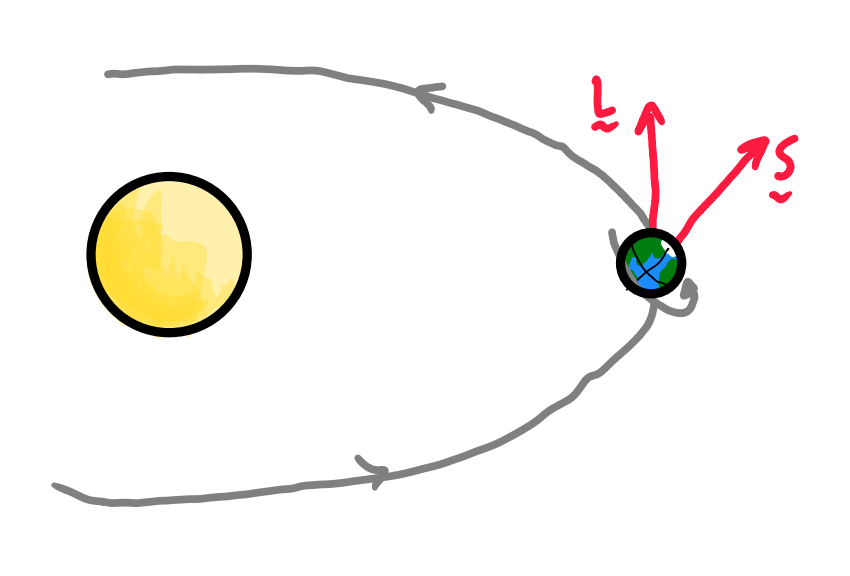
\includegraphics[width=0.5\linewidth]{Figures/Chapter 1/fig_sun_earth.png}
\caption{The Earth goes around the Sun every 365 days (orbital angular momentum) and rotates around its axis every 24 hours (spin angular momentum).}
\label{fig_sun_earth}
\end{figure}

As a simple quantum system, consider an electron in orbit around a proton -- a hydrogen atom.  The electron has orbital angular momentum just like the Earth (depending on what state it's in), and it also has spin angular momentum.  Careful, though, as the electron doesn't rotate like the Earth -- how can it when it has essentially no size or diameter to spin?  Despite this, it has measurable intrinsic angular momentum, which we'll call \emph{spin} $\vec{S}$.  Since spin is a vector, it has components $(S_x, S_y, S_z)$, and thus to specific the spin of the electron we use three different numbers; keep this in mind for later.

Suppose we put a stationary electron in a magnetic field $\vec{B}$.  Since the electron is stationary, the Lorentz force
\[
\vec{F} = q\vec{v} \times \vec{B}
\]
is zero.  But the electron's spin angular momentum gives it a magnetic dipole moment $\vec{\mu}$, and it's then possible for an \emph{inhomogeneous} magnetic field to exert a force (see Griffiths \emph{Introduction to Electrodynamics}, fourth edition, section 6.2)
\begin{equation}
\vec{F} = \grad (\vec{\mu} \cdot \vec{B}).
\end{equation}



%
%
%

\section{The Stern-Gerlach Experiment}

The 

%
%
%

\section{Extending the Experiments}

The 

%
%
%



\section*{Problems}
\addcontentsline{toc}{section}{Problems}
\markright{Problems}%

\begin{problem}[Electron spin]
How fast would the surface of an electron be going if it had ....
\end{problem}


\chapter{The Quantum State Vector}

\section{Basis States}

In the previous chapter I introduced the ket $\ket{\psi}$, and said that it represents a \emph{state} of a quantum mechanical system.  But what exactly is it?  It's hard to define, since by its nature it's abstract -- in some ways, it's meant to represent everything we could possibly know about a particular quantum system.  If we wanted to be technical I could tell you that it's a vector in complex Hilbert space, but I'm not sure that will help. Instead, I think it's best to draw an analogy with a vector space you know well:  vectors in three dimensional position space.  Before we do that, though, I want to also introduce a \emph{different} way of representing a quantum space, called (for reasons we'll see shortly) a ``bra'':
\begin{equation}
\label{eq_bra_definition}
\boxed{
\bra{\psi} \rightarrow \text{ Represents the state of a quantum mechanical system.}
}
\end{equation}
Our job in this chapter is to get at least a good working idea of what exactly a ket and bra actually are and how we use them in quantum mechanics.

I'm sure you recall some of the basics of how we write vectors -- that is, normal old vectors in Cartesian coordinates -- in physics.  We can use the unit vectors
\[
\hat{x}, \quad \hat{y}, \quad \hat{z}
\]
(or, if you prefer, $\hat{i}$, $\hat{j}$, and $\hat{k}$) to specify the three coordinate directions.  These unit vectors can be used to write any other vector in this coordinate system, so for example the vector $\vec{A}$ can be written as
\[
\vec{A} = A_x \hat{x} + A_y \hat{y} + A_z \hat{z},
\]
where $A_x$ and so on are the components of the vector along those directions.  The unit vectors are called \emph{complete} if they can be used to write every possible vector in this way.

In addition, these are \emph{unit} vectors, which means that have a length of exactly one (with no dimensions).  Mathematically we could express this using the dot product,
\[
\hat{x} \cdot \hat{x} = 1, \quad \hat{y} \cdot \hat{y} = 1, \quad \hat{z} \cdot \hat{z} = 1.
\]
We say that a vector is \emph{normalized} if this is the case -- that the dot product with itself is one.

Of course, these unit vectors are also \emph{orthogonal} -- they have 90$^\circ$ between them -- which we could also write in terms of dot products as
\[
\hat{x} \cdot \hat{y} = 0, \quad \hat{y} \cdot \hat{z} = 0, \quad \hat{z} \cdot \hat{x} = 0.
\]
Taken together, we can use the term \emph{orthonormal} for vectors that are both normalized and orthogonal.

The quantum state vectors $\ket{+}$ and $\ket{-}$ play a similar role as the unit vectors, but for spin-1/2 systems; because these states correspond to measuring spin up and spin down along the $z$ axis, these kets form the $S_z$ basis.  And like $\hat{x}$, $\hat{y}$, and $\hat{z}$), they're complete, so that any general spin-1/2 state can be written down in terms of them:
\begin{equation}
\ket{\psi} = a \ket{+} + b\ket{-}.
\end{equation}
The values $a$ and $b$ -- which can be complex numbers, so be careful -- in a loose sense\footnote{Careful with taking this too far; we'll see exactly what $a$ and $b$ tell us soon.} tell you how much of the general state $\ket{\psi}$ is made up of the spin up state ($a$) how much is made up of the spin down state ($b$).

Remember I introduced the bra $\bra{\psi}$ above?  Well, in the $S_z$ basis the state could also be written as
\begin{equation}
\bra{\psi} = a^* \bra{+} + b^* \bra{-}.
\end{equation}
Those stars indicate the \emph{complex conjugate}.  It's important to realize that not only are the two representations of the state -- the ket $\ket{\psi}$ and the bra $\bra{\psi}$ different -- one obviously involves the complex conjugate of the other -- but they're not even the same kind of mathematical object.  That said, either provides a full representation of the same state.

Okay, so what about these funny names, \emph{ket} and \emph{bra}?  They come about because of how we write the \emph{inner product} -- the analog to the dot product we used above for the unit vectors.  We stick the bra first, then the ket, like so:
\[
\braket{\text{bra}}{\text{ket}}.
\]
Can you see what the whole thing spells?  I think this is supposed to be a joke, so feel free to laugh; we're stuck with the notation, though, which Paul Dirac invented in 1939, and which we now call \emph{Dirac notation}. 

With the inner product defined, we can now write out the normalization condition for our basis vectors,
\begin{equation}
\braket{+}{+} = \braket{-}{-} = 1,
\end{equation}
as well as orthogonalization,
\begin{equation}
\braket{+}{-} = \braket{-}{+} = 0.
\end{equation}
Actually, in quantum mechanics, it's not just the basis vectors that are normalized; \emph{every} quantum state must be normalized:
\begin{equation}
\boxed{
\braket{\psi}{\psi} = 1.
}\end{equation}
I know I keep saying this, but we'll see why this must the case later.

\begin{example}[Normalization]  Consider the state 
\begin{equation}
\ket{\psi} = A \left( \ket{+} + 2i \ket{-} \right).
\end{equation}

Is the state normalized?  Check:
\begin{align*}
\braket{\psi}{\psi} &= 1 \\
\Rightarrow A^* \left( \bra{+} - 2i \bra{-} \right) \ A \left( \ket{+} + 2i\ket{-} \right) &=  1
\end{align*}
Expanding out the brackets, using the orthonormality conditions above, gives
\begin{equation}
\label{eq_norm}
5 |A|^2 = 1,
\end{equation}
where $|A|^2 \equiv A^* A$ is the ``complex square''.  Now, the complex square will always be a real number, which we can see easily if we write the the general complex number $A$ in polar form as
\[
A = r e^{i\theta},
\]
where $r$ (the \emph{amplitude}) and $\theta$ (the \emph{phase}) are both real numbers.  Then 
\[
|A|^2 = A^* A = re^{-i\theta} r e^{i\theta} = r^2.
\]
That means the normalization condition above in equation (\ref{eq_norm}) can't give us any information about the phase $\theta$, only the amplitude.  As it will turn out, that's okay -- an overall phase in a quantum state doesn't mean anything physically, and we'll see why in due time -- so by convention we take it to be zero, and set the constant to 
\[
A = \frac{1}{\sqrt{5}}.
\]
With this value of $A$, the state is normalized.
\end{example}

\begin{example}[Inner products]  Consider another state given by
\begin{equation}
\ket{\phi} = \frac{3}{5} \ket{+} - \frac{4}{5} \ket{-}.
\end{equation}
Notice that this state is already normalized (check it!).  What is the inner product between state $\ket{\psi}$ and $\ket{\phi}$?

Using Dirac notation we can write each state in their $S_z$ basis and ``foil'' it out to get
\begin{align*}
\braket{\psi}{\phi} & =  \left( \frac{1}{\sqrt{5}}\bra{+} - \frac{2i}{\sqrt{5}} \bra{-} \right) \left(\frac{3}{5} \ket{+} - \frac{4}{5} \ket{-} \right) \\
& = \frac{3}{5\sqrt{5}} + \frac{8i}{5\sqrt{5}}.
\end{align*}

Notice what happens if we reverse the order of the inner product:
\begin{align*}
\braket{\phi}{\psi} & =   \left(\frac{3}{5} \bra{+} - \frac{4}{5} \bra{-} \right) \left( \frac{1}{\sqrt{5}}\ket{+} + \frac{2i}{\sqrt{5}} \ket{-} \right) \\
& = \frac{3}{5\sqrt{5}} - \frac{8i}{5\sqrt{5}}.
\end{align*}
This is precisely the complex conjugate of the first inner product; in fact, in general for any two state vectors $\ket{\alpha}$ and $\ket{\beta}$ we have
\begin{equation}
\braket{\alpha}{\beta} = \braket{\beta}{\alpha}^*.
\end{equation}
\end{example}

\section*{Problems}
\addcontentsline{toc}{section}{Problems}
\markright{Problems}%

\begin{problem}[Electron spin]
This whole chapter is about electron spin, but of course the electron doesn't really spin around like a top.  But let's pretend for a moment that an electron really is a tiny sphere, of radius
\[
r_e = \frac{e^2}{4\pi \epsilon_0 mc^2}
\]
(the so-called classical electron radius), and that it spins around its axis with angular momentum $S_z = \hbar/2$.  How fast would a point on the ``equator'' be moving?  Does this model make sense? 
\end{problem}


\chapter{Amplitude and Probability}

\section{The $S_x$ and $S_y$ Spin States}

\section{Calculating Probability}

\section{The Stern-Gerlach Experiments Revisited}

\section{Indeterminant States}

\section*{Problems}
\addcontentsline{toc}{section}{Problems}
\markright{Problems}%

\begin{problem}[Spin-1/2 States]
Consider these different spin-1/2 states, given in Dirac notation by
\begin{align*}
\ket{\psi_1} &= 3 \ket{+} + 4\ket{-} \\
\ket{\psi_2} &= \ket{+} + 2i \ket{-} \\
\ket{\psi_3} &= 3 \ket{+} - e^{i\pi/3}\ket{-} \\
\ket{\psi_4} &= 3 \ket{+} - 5i\ket{-}.
\end{align*}
\begin{enumerate}[label=(\alph*)]
\item Normalize each state.
\item Write each state in matrix notation.
\item Write the bra of each ket; write the bras in matrix notation, too.
\item Find a (normalized) ket that is orthogonal to each state.
\item Compute the following inner products, using either Dirac notation or matrix notation:  $\braket{\psi_1}{\psi_2}$, $\braket{\psi_3}{\psi_4}$, $\braket{\psi_4}{\psi_1}$, and $\braket{\psi_3}{\psi_2}$.
\end{enumerate}
\end{problem}


\begin{problem}[A Three-State System]
So far we've only looked at the fairly simple two-state spin-1/2 system.  For this problem, consider a system which has \emph{three} orthonormal basis states, given by
\[
\ket{a_1}, \ket{a_2}, \text{ and }  \ket{a_3}.
\]
\begin{enumerate}[label=(\alph*)]
\item What would these kets look like in matrix notation?
\item Normalize the state
\[
\ket{\psi_1} = \ket{a_1} - 2 \ket{a_2} + 5 \ket{a_3}.
\]
\item Take the inner product of $\ket{\psi_1}$ with the state 
\[
\ket{\psi_2} = i\ket{a_1} + 3 \ket{a_2} - 2\ket{a_3}.
\]
(you'll have to normalize that state first, of course).
\end{enumerate}
\end{problem}


\chapter{Observables and Operators}

\section{Operators and Measurement}

We've already seen lots of examples of \emph{observables} -- the spin components $S_x$, $S_y$, and $S_z$ are all examples of things that we can observe, as are things like position and momentum.  In the language of quantum mechanics: 
\[
\boxed{\text{A physical observable $A$ is represented by an operator $\hat{A}$.}}
\]

Wait, what exactly is an operator?  At the risk of being too simplistic, it's something that \emph{operates} on a quantum state, producing a new state.  Mathematically we can write this operation like
\begin{equation}
\hat{A} \ket{\psi} = \ket{\phi}.\footnote{Although the hat on the operator is standard, many textbooks drop it to reduce clutter in notation.  I think it's important to be able to easily distinguish an observable and an operator at a glance, especially for newcomers.}
\end{equation}
Actually, although in general the operator $\hat{A}$ produces a new state, sometimes the state it operates on is special and \emph{doesn't} change:
\begin{equation}
\label{eq_eigen}
\hat{A} \ket{\psi} = a \ket{\psi}.
\end{equation}
Instead of making a new state, it gives back the same state, but multiplied by a number $a$.  If you're familiar with linear algebra, you might recognize equation (\ref{eq_eigen}) as an \emph{eigenvalue equation}, with $a$ playing the role of the eigenvalue and the ket $\ket{\psi}$ being the eigenvector.   The eigenvalue is very important:
\\

\fbox{
  \parbox{0.9\textwidth}{
    The only possible result of a measurement of an observable $A$ is one of the eigenvalues $a_n$ of the corresponding operator $\hat{A}$.
  }
}

\subsection{The Operator $\hat{S_z}$}

That's a lot to take in on first reading, so let's do a full example.  We'll return to the observable $S_z$, which must have a corresponding operator $\hat{S}_z$.  We'll figure out how we can write this in a moment, but you might have realized we already know the eigenvalues of this operator: they must be $\hbar/2$ and $-\hbar/2$, since we know measurements of $S_z$ always return one of those two numbers.

That means that the eigenvalue equations -- two of them for two eigenvalues -- could be written as
\begin{equation}
\hat{S}_z \ket{+} = \frac{\hbar}{2} \ket{+} \quad \text{and} \quad \hat{S}_z \ket{-} = -\frac{\hbar}{2} \ket{-}.
\end{equation}
We can get a sense of what the operator $\hat{S}_z$ is by thinking of this in matrix notation -- the states $\ket{+}$ and $\ket{-}$ are column vectors, meaning $\hat{S}_z$ must be represented as a $2\times 2$ matrix (nothing else, when multiplied by a column vector, gives another column vector).  I don't know what the elements of the matrix are, so I'll write it out for now as
\[
\hat{S}_z \to \begin{pmatrix} a & b \\ c & d \end{pmatrix}.
\]

To find the unknown elements $a$, $b$, $c$, and $d$ (which could be complex), we can go back to the eigenvalue equations, this time in matrix notation.  For the eigenvalue $\hbar/2$, we have
\begin{equation}
\hat{S}_z \ket{+} = \frac{\hbar}{2} \ket{+} \to \begin{pmatrix} a & b \\ c & d \end{pmatrix} \begin{pmatrix} 1 \\ 0 \end{pmatrix} = \frac{\hbar}{2} \begin{pmatrix} 1 \\ 0 \end{pmatrix}.
\end{equation}
Multiplying out the left side gives
\[
\begin{pmatrix} a \\ c \end{pmatrix} = \begin{pmatrix} \hbar/2 \\ 0 \end{pmatrix},
\]
so we know that $a = \hbar/2$ and $c = 0$.  The other eigenvalue equation, for $-\hbar/2$, similarly gives $b = 0$ and $d = -\hbar/2$.  The operator $\hat{S}_z$, in matrix notation, is
\begin{equation}
\hat{S}_z \to \frac{\hbar}{2} \begin{pmatrix} 1 & 0 \\ 0 & -1 \end{pmatrix}.
\end{equation}

There's a few things here we should notice -- in particular that $\hat{S}_z$ is a \emph{diagonal} matrix, with the eigenvalues as the diagonal elements.  Also note that the eigenvectors (the states $\ket{+}$ and $\ket{-}$) are unit vectors.  Both of these things arise because of the basis were using -- it's the $S_z$ basis!  In other words, in its own basis -- where the basis states are the eigenstates of the basis operator -- an operator will be diagonal with the eigenvalues along that diagonal.

\section{Matrix Representation}

In fact, any operator can be represented as a matrix; sticking with the $S_z$ basis, we can write a general operator $\hat{A}$ as a $2 \times 2$ matrix
\begin{equation}
\hat{A} \to \begin{pmatrix} a & b \\ c & d \end{pmatrix}.
\end{equation}

Now for something a little new.  Consider the calculation $\bra{+} \hat{A} \ket{+}$.  What exactly does this mean?  First we apply the operator $\hat{A}$ to the ket $\ket{+}$, getting a new state, and then apply the bra $\bra{+}$ to that new state:
\[
\bra{+} \Big( \hat{A} \ket{+} \Big) \to \begin{pmatrix} 1 & 0 \end{pmatrix} \begin{pmatrix} a & b \\ c & d \end{pmatrix} \begin{pmatrix} 1 \\ 0 \end{pmatrix} = \begin{pmatrix} 1 & 0 \end{pmatrix} \begin{pmatrix} a \\ b \end{pmatrix} = a.
\]
So the ultimate result is just a number -- $a$ in this case.  Similarly, you can show that $\bra{+}\hat{A} \ket{-} = b$, and so on.  That means we could be able to write our operator in matrix notation as
\begin{equation}
\hat{A} \to \begin{pmatrix} \bra{+}\hat{A}\ket{+} & \bra{+}\hat{A}\ket{-} \\ \bra{-}\hat{A}\ket{+} & \bra{-}\hat{A}\ket{-} \end{pmatrix}.
\end{equation}
This is just notation, but useful since we can see explicitly what the basis is.

It's easy enough to generalize this to any system; the matrix representation might have a different size than $2 \times 2$ (it might even be infinite), but the idea is the same.  In general we can write
\begin{equation}
\hat{A} \to \begin{pmatrix} 
a_{11} & a_{12} & a_{13} & \cdots \\ 
a_{21} & a_{22} & a_{23} & \cdots \\
a_{31} & a_{32} & a_{33} & \cdots \\
\vdots & \vdots & \vdots  & \ddots
\end{pmatrix},
\end{equation}
where $a_{ij} = \bra{i} \hat{A} \ket{j}$ and $\ket{i}$ and $\ket{j}$ are the basis states.  In this context we'll often call the $a_{ij}$s matrix elements.


\section{The Operators $\hat{S}_x$ and $\hat{S}_y$}

The matrix representation of the other two spin component operators are given by
\begin{equation}
\hat{S}_x \to \frac{\hbar}{2} \begin{pmatrix} 0 & 1 \\ 1 & 0 \end{pmatrix}
\end{equation}
and 
\begin{equation}
\hat{S}_y \to \frac{\hbar}{2} \begin{pmatrix} 0 & -i \\ i & 0 \end{pmatrix}.
\end{equation}
These are both written in the $S_z$ basis (notice that they're not diagonal).  If you'd like to know where these came from, feel free to work through the Stern-Gerlach results in Problem XXX.  What I'd rather do right now is ask the question: \emph{if we were to measure, say, $S_y$ on some particular state, what are the possible results we could get?}  We already know the answer in this case, but a lot of quantum mechanics boils down to figuring out the answer to this question for a variety of different observables and corresponding operators, so it's worth going through the process in detail.

The answer, as mentioned above, is given by the eigenvalues of the operator. You probably already know how to find eigenvalues fro your linear algebra course, but let's do it together nice and slow.  First, the eigenvalue equation is
\begin{equation}
\label{eq_eigeny}
\hat{S}_y \ket{\lambda} = \lambda \ket{\lambda},
\end{equation}
where $\lambda$ does double duty here, standing for the unknown eigenvalue as well as the corresponding eigenstate.  This might seem confusing at first, but we'll get used to it. 

We find the eigenvalues by solving the characteristic (or secular) equation , which looks like
\begin{equation}
\det | \textbf{S}_y - \lambda \textbf{I} | = 0.
\end{equation}
The bolded letter $\textbf{S}_y$ denote the matrix representation of the operator, and $\textbf{I}$ is the identity matrix.  Filling in the matrices gives
\[
\left| \begin{pmatrix} 0 & -i\hbar/2 \\ i\hbar/2 & 0  \end{pmatrix} - \begin{pmatrix} \lambda &  0 \\ 0 & \lambda \end{pmatrix} \right| = 0,
\]
or, after simplifying,
\[
\left| \begin{pmatrix} -\lambda & -i\hbar/2 \\ i\hbar/2 & -\lambda  \end{pmatrix} \right| = 0.
\]
Work out the determinant to get
\[
\lambda^2 - \left( \frac{\hbar}{2} \right)^2 = 0
\]
so that, finally, we can see that the two eigenvalues -- as expected! -- are $\lambda_1 = \hbar/2$ and $\lambda_2 = -\hbar/2$.  These two values are the only possible results we would get if we measured $S_y$ on any spin state.

What about the eigenstates?  To find these, we go back to the original eigenvalue equation (\ref{eq_eigeny}) and plug in each eigenvalue in turn.  For $\lambda = \hbar/2$, we have
\[
\hat{S}_y \ket{\lambda} = \frac{\hbar}{2} \ket{\lambda}.
\]
Writing the unknown state $\ket{\lambda}$ in matrix notation,
\begin{equation}
\ket{\lambda} \to \begin{pmatrix} \alpha \\ \beta \end{pmatrix},
\end{equation}
our job is to find the value of $\alpha$ and $\beta$ that satisfy the eigenvalue equation.  Here we go:
\[
\hat{S}_y \ket{\lambda} = \frac{\hbar}{2} \ket{\lambda} \to 
\frac{\hbar}{2} \begin{pmatrix} 0 & -i \\ i & 0 \end{pmatrix} \begin{pmatrix} \alpha \\ \beta \end{pmatrix} = 
\frac{\hbar}{2}  \begin{pmatrix} \alpha \\ \beta \end{pmatrix},
\]
so
\[
\begin{pmatrix} -i \beta \\ i\alpha \end{pmatrix} =  \begin{pmatrix} \alpha \\ \beta \end{pmatrix}.
\]
This is really two equations for $\alpha$ and $\beta$, but they're the same equation -- we don't have enough information to get both values right now.  But we can at least solve for $\beta$ in terms of $\alpha$ and get
\[
\beta = i \alpha,
\]
making the eigenstate so far
\begin{equation}
\ket{\lambda} = \ket{+}_y \to \alpha \begin{pmatrix} 1 \\ i \end{pmatrix}.
\end{equation}
How, then, do we get the last unknown $\alpha$?  Well, every state must be normalized, so
\begin{equation}
_y \braket{+}{+}_y = 1. 
\end{equation}
In matrix notation, this becomes
\[
|\alpha|^2 \begin{pmatrix} 1 & -i \end{pmatrix} \begin{pmatrix} 1 \\ i \end{pmatrix} = |\alpha|^2 (2) = 1,
\]
so we'll take
\[
\alpha = \frac{1}{\sqrt{2}}
\]
and therefore
\begin{equation}
\ket{+}_y = \frac{1}{\sqrt{2}} \ket{+} + \frac{i}{\sqrt{2}} \ket{-} \to \frac{1}{\sqrt{2}} \begin{pmatrix} 1 \\ i \end{pmatrix}.
\end{equation}

Feel free to go through the same process to get the spin down eigenstate; it turns out to be
\begin{equation}
\ket{-}_y = \frac{1}{\sqrt{2}} \ket{+} - \frac{i}{\sqrt{2}} \ket{-} \to \frac{1}{\sqrt{2}} \begin{pmatrix} 1 \\ -i \end{pmatrix}.
\end{equation}
Problem XXX will get you to go through the process for $S_x$.



\section{Spin in a General Direction, $\hat{S}_n$}

At this point I just want to give you some more operators and figure out their eigenvalues and eigenstates, partly so we can get the practice and partly so we can use them again later.  First up, suppose we rotate our usual Stern-Gerlach device to some random orientation so that the magnetic field points in the direction of $\vec{n}$ as shown in Figure XXX.  The angles $\theta$ (the polar angle) and $\phi$ (the azimuthal angle) are the usual spherical coordinates, and we'll make $\vec{n}$ a unit vector so it has a length of one.  That means in terms of the Cartesian unit vectors $\unit{x}$, $\unit{y}$, and $\unit{z}$, we can write
\begin{equation}
\vec{n} = \sin \theta \cos \phi \, \unit{x} + \sin \theta \sin \phi \, \unit{y} + \cos \theta \, \unit{z}.
\end{equation}

Suppose we measure the spin of a particle along this direction; let's call the observable $S_n$, where
\begin{equation}
S_n = \vec{S} \cdot \vec{n} = S_x \sin \theta \cos \phi  + S_y \sin \theta \sin \phi + S_z \cos \theta.
\end{equation}
The operator associated with this observable is, of course, the exact same except with hats on the operators, so we have\footnote{Okay, we have to be a little careful now distinguishing unit vectors from operators, both of which have hats.  Things should be clear from context.}
\begin{equation}
\hat{S}_n = \hat{\vec{S}} \cdot \vec{n} = \hat{S}_x \sin \theta \cos \phi  + \hat{S}_y \sin \theta \sin \phi  + \hat{S}_z \cos \theta.
\end{equation}
To write this operator in matrix notation, we just fill in the matrices for $\hat{S}_x$, $\hat{S}_y$, and $\hat{S}_z$ and add them together to get
\begin{equation}
\hat{S}_n \to \frac{\hbar}{2} \begin{pmatrix} \cos \theta & \sin \theta \, e^{-i\phi} \\ \sin \theta \, e^{i\phi} & -\cos \theta \end{pmatrix}
\end{equation}
(see Problem XXX).

This is a new operator we've never seen before, and anytime we're faced with a new operator, we should always find its eigenvalues and eigenstates -- remember, the eigenvalues of the operator answer the question of what we get when we measure the observable, so they're pretty important, and we'll see that the eigenstates play just as important a role.  But wait -- we \emph{already} know the eigenvalues!  They \emph{have} to be $\hbar/2$ and $-\hbar/2$, just like $\hat{S}_x$ or any other component.  After all, changing the direction of the magnetic field by rotating the device is the exact same operation as changing our coordinate system, and that should affect the actual results we get.

So, fine, we know the eigenvalues (you can check that we're correct in Problem XXX); what about the eigenstates?  You need more practice than I do, so try on your own (that's Problem XXX again), and I'll give you just the answers for now.  The eigenstates are (with notation that should be clear by now; the ket $\ket{+}_n$ is the state that goes with $+\hbar/2$ and similarly for the eigenvalue $-\hbar/2$)
\begin{equation}
\ket{+}_n = \cos (\theta/2) \, \ket{+} + \sin (\theta/2) \, e^{i\phi} \, \ket{-}
\end{equation}
and
\begin{equation}
\ket{-}_n = \sin (\theta/2) \, \ket{+} - \cos (\theta/2) \, e^{i\phi} \, \ket{-}.
\end{equation}
Remember, all this is explicitly in the $S_z$ basis.

By the way, if you were wondering how we make some ``general spin state'' $\ket{\psi}$ with some specific set of coefficients, this is how:  orient the Stern-Gerlach device at just the correct angles $\theta$ and $\phi$ that give you those coefficients.  Problem XXX will ask you to do this.

\section*{Problems}
\addcontentsline{toc}{section}{Problems}
\markright{Problems}%

\begin{problem}[Orthogonality]
Show that the states $\ket{+}_x$ and $\ket{-}_x$ are orthogonal.  Do the same for the states $\ket{+}_y$ and $\ket{-}_y$. 
\end{problem}



\chapter{Examples of Discrete Systems}

\section{An Electron in a Magnetic Field}

To come.
%
%
%

\section{Neutrino Oscillations}

Neutrinos -- little neutral particles created in huge numbers during nuclear reactions -- were long though to be massless.  But during the 1980s and 1990s the \emph{solar neutrino problem} became undeniable: neutrino detection experiments on Earth were missing about half of the expected number of neutrinos made in the core of the sun during hydrogen burning.  There were only two possibilities:  either our model of the sun was way off\footnote{One of my undergraduate professors was a solar physicists, and according to him there was no way the solar models could be that wrong, so really there's only one possible explanation -- something was wrong with our understanding of neutrinos.} or something happened to the neutrinos on their way to us.

The correct explanation turned out to be something called \emph{neutrino oscillations}, and the theory earned the Nobel prize.  In short, \emph{electron} neutrinos are created in the core of the sun, but on their way to Earth some of them turn into \emph{muon} neutrinos -- don't worry too much about the names or why there's more than one kind of neutrino; the main idea is that neutrinos can oscillate back and forth between these two different types (actually, there's a \emph{third} type, a tau neutrino, but we'll ignore that for simplicity).

As a slightly simplified model for neutrino mixing, we'll suppose the state of any neutrino -- I'll call this the ``flavour state,'' since particle physicists call the type of particle its flavour for some reason -- can be written as a superposition of an electron neutrino state and a muon neutrino state:
\begin{equation}
\ket{\nu} = a \ket{e} + b \ket{\mu}.
\end{equation}
This is a two-state system, something we've already studied in detail, so the physics of neutrinos is pretty much the same as spin-1/2 systems or photon polarizations.  To see how neutrinos oscillate, though, we'll have to calculate how this state evolves in time, meaning we'll need the Hamiltonian of the system.

The Hamiltonian, of course, is just the total energy, so we'll start with the relativistic energy of any particle (unfortunately, neutrinos are inherently relativistic objects -- it's hard to slow them down), 
\[
E = \sqrt{p^2c^2 + m^2 c^4}.
\]
Although neutrinos were originally thought to be massless, it turns out we'll need to give them a very small mass in order for them to oscillate.  That said, it will be a \emph{very} small mass, so it's reasonable to think that their rest energy ($mc^2)$ will be much smaller than their momentum (the $pc$ term), in which case we can write 
\[
E = pc \left( 1 + \frac{m^2c^4}{p^2c^2} \right)^{1/2} \approx pc \left( 1 + \frac{m^2c^4}{2p^2c^2} \right),
\]
or
\begin{equation}
\label{eq_relE}
E = pc + \frac{m^2c^3}{2p}.
\end{equation}
For reasons we won't see until we solve the whole problem, I'm going to write the Hamiltonian as
\begin{equation}
\hat{H} \to \begin{pmatrix}
pc + (m_1^2 + m_2^2) c^3/4p & (m_1^2 - m_2^2)c^3/4p \\
(m_1^2 - m_2^2)c^3/4p &pc + (m_1^2 + m_2^2) c^3/4p 
\end{pmatrix}
\end{equation}
where $m_1$ and $m_2$ are two different masses.  You might think that $m_1$ is the mass of the electron neutrino and $m_2$ is that of the muon neutrino, but that's not quite the case; hold tight and we'll see what that means.

Before we find the energy eigenvalues and eigenstates, consider for a moment what the Hamiltonian would look like if the neutrinos were in fact \emph{massless}; then
\[
\hat{H} \to \begin{pmatrix}
pc & 0 \\
0 & pc 
\end{pmatrix}.
\]
This matrix is diagonal, so the possible energies are easy to read off: they're both the same, $E = pc$ as we'd expect for a massless relativistic particle.  The eigenstates of the matrix are just the flavour basis states, $\ket{e}$ and $\ket{\mu}$, so the implication is that both neutrinos have the same energy.  More importantly, though, the flavour states -- which are also the energy eigenstates -- are stationary states, so neutrino oscillations simply wouldn't happen.  Once an electron neutrino is created during a reaction, it will stay an electron neutrino forever.  Actually, it's possible to have massive neutrinos and still have the flavour states be stationary, as long as the masses are the same.  In this case the matrix remains diagonal and we reach the same conclusions; evidently it's the \emph{different} masses of the two neutrinos that lead to oscillations.

Okay, let's find the energies of the full Hamiltonian.  For ease of writing stuff out, I'm going to write the Hamiltonian as
\[
\hat{H} \to \begin{pmatrix}
h & g \\
g & h 
\end{pmatrix},
\]
where $h = pc + (m_1^2 + m_2^2) c^3/4p$ and $g = (m_1^2 - m_2^2)c^3/4p$.  The characteristic equation is
\[
\begin{vmatrix}
h - E & g \\
g & h - E
\end{vmatrix} = 0,
\]
which has solutions
\begin{equation}
E_1 = h + g = pc + (m_1^2 + m_2^2) c^3/4p + (m_1^2 - m_2^2)c^3/4p = pc + m_1^2 c^3 / 2p
\end{equation}
and
\begin{equation}
E_2 = h - g = pc + (m_1^2 + m_2^2) c^3/4p - (m_1^2 - m_2^2)c^3/4p = pc + m_2^2 c^3 / 2p.
\end{equation}
Now you can see why I chose the exact Hamiltonian I did -- we get exactly the energies we expect based on equation \ref{eq_relE}.  As long as the masses are different, these are two distinct energies.

Now that we have the energy eigenvalues, we can get the corresponding states as well.  For $E = E_1 = h + g$, the eigenvalue equation is
\[
\hat{H} \ket{E_1} = E_1 \ket{E_1},
\]
or, in matrix notation,
\[
\begin{pmatrix}
h & g \\
g & h
\end{pmatrix} \begin{pmatrix}  \alpha \\ \beta \end{pmatrix} = (h+g) \begin{pmatrix}  \alpha \\ \beta \end{pmatrix}.
\]
Solving gives $\beta = \alpha$, and after normalizing to find $\alpha = 1/\sqrt{2}$, the eigenstate is 
\begin{equation}
\label{eq_E1}
\ket{E_1} = \frac{1}{\sqrt{2}} \ket{e} + \frac{1}{\sqrt{2}} \ket{\mu}.
\end{equation}
Similarly, the eigenstate associated with energy $E_2 = h - g$ is
\begin{equation}
\label{eq_E2}
\ket{E_2} = \frac{1}{\sqrt{2}} \ket{e} - \frac{1}{\sqrt{2}} \ket{\mu}.
\end{equation}


This is where things get interesting and a little weird.   According to particle physics, a neutrino is created either as an electron neutrino (state $\ket{e}$) or as a muon neutrino (state $\ket{\mu}$).  But the energy states are a superposition of these flavour states -- evidently the electron neutrino, say, just doesn't \emph{have} a definite energy.  Put another way -- because the energies depend on the two different masses -- we can say the an electron neutrino does not have a definite mass; the $m_1$ isn't an $m_{\nu_e}$.  Alternatively, if we manage to measure the energy (or mass) of an electron neutrino, it's no longer an electron neutrino -- its state collapses to one of the superpositions above and it doesn't have a definite flavour.

We can see how this leads to neutrino oscillations and solves the solar neutrino problem by supposing that, at the centre of the sun, an electron neutrino is created.  The initial state is then
\begin{equation}
\ket{\nu(0)} = \ket{e}.
\end{equation}
I think it's fair to call this neutrino an electron neutrino at this point.

To find the state at a later time, we need to first switch to the energy basis.  For fun, I'll do that by multiplying the state by the identity operator:
\[
\ket{\nu(0)} = \hat{1} \ket{e} = \left( \ket{E_1}\bra{E_1} + \ket{E_2} \bra{E_2} \right) \ket{e}.
\]
Notice that I wrote the identity operator in the energy basis -- this is the mechanism that switches basis for us.  Working out the inner products gives
\begin{equation}
\ket{\nu(0)} =  \frac{1}{\sqrt{2}} \ket{E_1} + \frac{1}{\sqrt{2}} \ket{E_2}
\end{equation}
as you might expect; although it's fair to say this is an electron neutrino, we definitely can't say what the energy of the particle is -- it simply doesn't have one.

Now we can tack on the exponential time factors to find the state at a later time in the usual way.  We get
\[
\ket{\nu(t)} = \frac{e^{-iE_1 t / \hbar}}{\sqrt{2}} \ket{E_1} + \frac{e^{-iE_2 t / \hbar}}{\sqrt{2}} \ket{E_2}.
\]
Finally, I'll switch back to the flavour basis, although this time I'll do it using equations (\ref{eq_E1}) and (\ref{eq_E2}) directly rather than using the identity operator:
\[
\ket{\nu(t)} = \frac{e^{-iE_1 t / \hbar}}{\sqrt{2}} \left( \frac{1}{\sqrt{2}} \ket{e} + \frac{1}{\sqrt{2}} \ket{\mu} \right)  + \frac{e^{-iE_2 t / \hbar}}{\sqrt{2}} \left( \frac{1}{\sqrt{2}} \ket{e} - \frac{1}{\sqrt{2}} \ket{\mu} \right).
\]
Using $E_1 = h + g$ and $E_2 = h -g$ and simplifying things, we get
\[
\ket{\nu(t)} = \frac{1}{2} e^{-iht/\hbar} \left[  \left( e^{-igt/\hbar} + e^{igt/\hbar} \right) \ket{e} +  \left( e^{-igt/\hbar} - e^{igt/\hbar} \right) \ket{\mu} \right].
\]
You might recognize cosine and sine in there, so we'll simplify further, but also note that there's an overall phase factor out in front -- we'll drop that since it doesn't mean anything physically.  Finally, the state at time $t$ is
\begin{equation}
\ket{\nu(t)} = \cos (gt/\hbar) \ket{e} - i \sin(gt/\hbar) \ket{\mu}.
\end{equation}
Take a look at what happens at time
\[
\tau = \frac{\pi \hbar}{g} = \frac{\pi p \hbar}{4c^3} \frac{1}{m_1^2 - m_2^2};
\]
at that point the cosine term goes to zero and the sine term becomes one and our state is
\[
\ket{\nu(\tau)} = \ket{\mu}.
\]
The electron neutrino has oscillated into a muon neutrino!

This is the explanation for the solar neutrino problem, although the full theory is a bit more complex since there are actually three different neutrino flavours.  But the main idea is still the same -- the flavour states are not the energy eigenstates, and are therefore not stationary -- they instead oscillate amongst themselves.



%
%
%



\chapter{The Finite Square Well}

\section{Bound States}

What happens if the walls of our ``box'' weren't quite so high?  Let's find out -- suppose we have a particle in a \emph{finite} square well, defined by the potential energy
\begin{equation}
V(x) = \begin{cases}
V_0, \quad x<-a \\
0, \quad -a<x<a \\
V_0, \quad x>a,
\end{cases}
\end{equation}
where $V_0$ is a positive constant -- the depth of the well as shown in Figure \ref{fig_finite_sqr_well_potential}.  Notice one other difference from the infinite version as well: the well has been centered at $x=0$ so the width of the well is actually $2a$; we'll see why in a little bit. 

\begin{figure}
\centering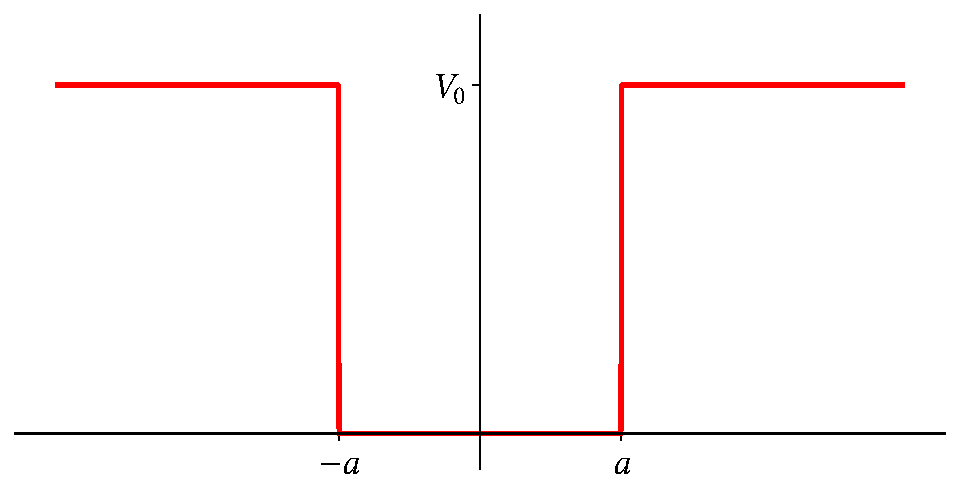
\includegraphics[width=0.7\linewidth]{Figures/Chapter 10/fig_finite_sqr_well_potential.pdf}
\caption{The potential energy of the finite square well.}
\label{fig_finite_sqr_well_potential}
\end{figure}

Actually, probably the biggest difference between the infinite square well and the finite well is what kind of states are allowed.  Classically, for the infinite square well, the particle in the box was always contained and could never escape, regardless of the energy of the particle.  In the finite well, though, if $E>V_0$ the particle would not be trapped in the box and would instead escape to infinity.  As we discussed back in Chapter 8, this case would be an \emph{unbound state}, and unbound states have some additional complications in quantum mechanics -- we'll save those for a later chapter.  In the meantime, we'll only look for bound energy eigenstates, where
\[
E < V_0 \quad \text{(bound states)},
\]
but keep in mind that we'll be missing some of the eigenstates.  One consequence of this is that the energy eigenstates we find here won't be \emph{complete}.

Luckily, finding the bound states is pretty easy.  For $x < -a$, to the left of the well, the energy eigenvalue equation reads
\[
-\frac{\hbar^2}{2m} \frac{d^2 \phi}{dx^2} + V_0 \phi = E\phi,
\]
or, cleaning it up a bit,
\begin{equation}
\frac{d^2\phi}{dx^2} = q^2 \phi,
\end{equation}
where
\begin{equation}
q = \frac{\sqrt{2m(V_0 - E)}}{\hbar}.
\end{equation}
Notice that $q$ is always \emph{real} since we're requiring that $E<V_0$.  This should be a recognizable differential equation; the general solution looks like
\begin{equation}
\phi(x) = A e^{qx} + B e^{-qx} \quad \text{($x<-a$)}.
\end{equation}
Similarly, for $x>a$, the potential energy is again $V = V_0$ so our solution is the same, although we'll have to use different constants:
\begin{equation}
\phi(x) = F e^{qx} + G e^{-qx} \quad \text{($x>a$)}.
\end{equation}

Finally, in the well itself we have $V = 0$, so the solution is the exact same as the infinite square well.  We can write the energy eigenvalue equation as
\begin{equation}
\frac{d^2\phi}{dx^2} = -k^2 \phi,
\end{equation}where
\begin{equation}
k = \frac{\sqrt{2mE}}{\hbar}
\end{equation}
is once again real and positive.  The general solution is 
\begin{equation}
\phi(x) = C \sin(kx) + D\cos(kx) \quad \text{($-a<x<a$)}.
\end{equation}

At the risk of repeating myself unnecessarily, I'll write out the full solution as a piecewise function; it helps to see it all together:
\begin{equation}
\phi(x) = \begin{cases}
A e^{qx} + B e^{-qx}, \quad & x<-a \\
C \sin(kx) + D\cos(kx) , \quad & -a<x<a \\
 F e^{qx} + G e^{-qx}, \quad & x>a.
\end{cases}
\end{equation}
Now all we have to do is find all six constants $A$, $B$, $C$, $D$, $F$, and $G$, plus of course our allowed energy $E$, which is buried inside $q$ and $k$.  To do that we use \emph{boundary conditions} as usual.

%
%
%

\section{Boundary Conditions}





\end{document}
